
%% bare_lsens.tex
%% V1.0
%% 2017/07/12
%% by Michael Shell
%% see http://www.michaelshell.org/
%% for current contact information.
%%
%% This is a skeleton file demonstrating the use of IEEE_lsens.cls for
%% an IEEE Sensors Letters paper.
%%
%% Support sites:
%% -- LaTeX Related --
%% http://www.michaelshell.org/tex/ieeetran/
%% http://www.ctan.org/pkg/ieeetran/
%%
%% -- IEEE/Editor/Submission Related --
%% http://www.ieee-sensors.org/
%% http://www.ieee.org/


%%*************************************************************************
%% Legal Notice:
%% This code is offered as-is without any warranty either expressed or
%% implied; without even the implied warranty of MERCHANTABILITY or
%% FITNESS FOR A PARTICULAR PURPOSE! 
%% User assumes all risk.
%% In no event shall the IEEE or any contributor to this code be liable for
%% any damages or losses, including, but not limited to, incidental,
%% consequential, or any other damages, resulting from the use or misuse
%% of any information contained here.
%%
%% All comments are the opinions of their respective authors and are not
%% necessarily endorsed by the IEEE.
%%
%% This work is distributed under the LaTeX Project Public License (LPPL)
%% ( http://www.latex-project.org/ ) version 1.3, and may be freely used,
%% distributed and modified. A copy of the LPPL, version 1.3, is included
%% in the base LaTeX documentation of all distributions of LaTeX released
%% 2003/12/01 or later.
%% Retain all contribution notices and credits.
%% ** Modified files should be clearly indicated as such, including  **
%% ** renaming them and changing author support contact information. **
%%*************************************************************************
% *** Authors should verify (and, if needed, correct) their LaTeX system  ***
% *** with the testflow diagnostic prior to trusting their LaTeX platform ***
% *** with production work. The IEEE's font choices and paper sizes can   ***
% *** trigger bugs that do not appear when using other class files.       ***
% The testflow support page is at:
% http://www.michaelshell.org/tex/testflow/
% Typically, there isn't any need for class options with IEEE Sensors
% Letters papers. The default, and only, text size is 9pt.
\documentclass{IEEE_lsens}
%
% If IEEE_lsens.cls has not been installed into the LaTeX system files,
% manually specify the path to it like:
% \documentclass{../sty/IEEE_lsens}
% *** Do not adjust lengths that control margins, column widths, etc. ***
% *** Do not use packages that alter fonts (such as pslatex).         ***
% There should be no need to do such things with IEEE_lsens.
% (Unless specifically instructed to do so by the IEEE Sensors Letters
% editors, of course.)
% Some very useful LaTeX packages include:
% (uncomment the ones you want to load)
% *** MISC UTILITY PACKAGES ***
%
%\usepackage{ifpdf}
% Heiko Oberdiek's ifpdf.sty is very useful if you need conditional
% compilation based on whether the output is pdf or dvi.
% usage:
% \ifpdf
%   % pdf code
% \else
%   % dvi code
% \fi
% The latest version of ifpdf.sty can be obtained from:
% http://www.ctan.org/pkg/ifpdf
% Also, note that IEEEtran.cls V1.7 and later provides a builtin
% \ifCLASSINFOpdf conditional that works the same way.
% When switching from latex to pdflatex and vice-versa, the compiler may
% have to be run twice to clear warning/error messages.
% The textcomp package can be loaded to get better \textcopyright and
% \textregistered symbols (as is used in the footer of the title page
% of LSENS papers).
\usepackage{textcomp}
% *** CITATION PACKAGES ***
%
\usepackage[noadjust]{cite}
% cite.sty was written by Donald Arseneau
% V1.6 and later of IEEEtran pre-defines the format of the cite.sty package
% \cite{} output to follow that of the IEEE. Loading the cite package will
% result in citation numbers being automatically sorted and properly
% "compressed/ranged". e.g., [1], [9], [2], [7], [5], [6] without using
% cite.sty will become [1], [2], [5]--[7], [9] using cite.sty. cite.sty's
% \cite will automatically add leading space, if needed. Use cite.sty's
% noadjust option (cite.sty V3.8 and later) if you want to turn this off
% such as if a citation ever needs to be enclosed in parenthesis.
% cite.sty is already installed on most LaTeX systems. Be sure and use
% version 5.0 (2009-03-20) and later if using hyperref.sty.
% The latest version can be obtained at:
% http://www.ctan.org/pkg/cite
% The documentation is contained in the cite.sty file itself.
% *** GRAPHICS RELATED PACKAGES ***
%
\ifCLASSINFOpdf
\usepackage{calc,amsmath,amssymb,amsfonts}
\usepackage[T1]{fontenc}
\usepackage[english]{babel}
\usepackage{xcolor,longfbox,fancyhdr}
\usepackage[top=1in,bottom=0.5in,hmargin=1in,nohead,includefoot,foot=0.5in,footskip=0.9602in]{geometry}
\usepackage{array,supertabular,hhline,enumitem,hyperref}


   \usepackage[pdftex]{graphicx}
  % declare the path(s) where your graphic files are
  % \graphicspath{{../pdf/}{../jpeg/}}
  % and their extensions so you won't have to specify these with
  % every instance of \includegraphics
   %\DeclareGraphicsExtensions{.pdf,.jpeg,.png}
\else
  % or other class option (dvipsone, dvipdf, if not using dvips). graphicx
  % will default to the driver specified in the system graphics.cfg if no
  % driver is specified.
  % \usepackage[dvips]{graphicx}
  % declare the path(s) where your graphic files are
  % \graphicspath{{../eps/}}
  % and their extensions so you won't have to specify these with
  % every instance of \includegraphics
  % \DeclareGraphicsExtensions{.eps}
\fi
% graphicx was written by David Carlisle and Sebastian Rahtz. It is
% required if you want graphics, photos, etc. graphicx.sty is already
% installed on most LaTeX systems. The latest version and documentation
% can be obtained at: 
% http://www.ctan.org/pkg/graphicx
% Another good source of documentation is "Using Imported Graphics in
% LaTeX2e" by Keith Reckdahl which can be found at:
% http://www.ctan.org/pkg/epslatex
%
% latex, and pdflatex in dvi mode, support graphics in encapsulated
% postscript (.eps) format. pdflatex in pdf mode supports graphics
% in .pdf, .jpeg, .png and .mps (metapost) formats. Users should ensure
% that all non-photo figures use a vector format (.eps, .pdf, .mps) and
% not a bitmapped formats (.jpeg, .png). The IEEE frowns on bitmapped formats
% for line art (i.e., plots, graphs, etc.) as they result in 
% "jaggedy"/blurry rendering of lines and letters as well as large
% increases in file sizes.
%
% You can find documentation about the pdfTeX application at:
% http://www.tug.org/applications/pdftex
% *** MATH PACKAGES ***
\usepackage[T1]{fontenc} % optional enhanced font encoding
\usepackage{amsmath}
% A popular package from the American Mathematical Society that provides
% many useful and powerful commands for dealing with mathematics.
%
% Note that the amsmath package sets \interdisplaylinepenalty to 10000
% thus preventing page breaks from occurring within multiline equations. Use:
\interdisplaylinepenalty=2500
% after loading amsmath to restore such page breaks as IEEEtran.cls normally
% does. amsmath.sty is already installed on most LaTeX systems. The latest
% version and documentation can be obtained at:
% http://www.ctan.org/pkg/amsmath

\usepackage[cmintegrals]{newtxmath}
% A Times compatible math font is required for IEEE Sensors Letters.
% Michael Sharpe's freely available newtxmath package (version 1.451,
% July 28, 2015 or later) is recommended. The cmintegrals option, which
% IEEE_lsens sets as a default upon loading newtxmath, is/was needed to
% obtain the specific style of integral symbol used by the IEEE Sensors
% Letters. However, as of version 1.5 of the newtxmath package, released
% on 2016/08/12, the correct integral symbol is now invoked by default
% and the cmintegrals option is no longer needed and is silently ignored.
% The latest version and documentation can be obtained at:
% http://www.ctan.org/pkg/newtx
\usepackage{bm}
% support for selective bold math 
% The latest version and documentation can be obtained at:
% http://www.ctan.org/pkg/bm

% *** SPECIALIZED LIST PACKAGES ***
%
%\usepackage{algorithmic}
% algorithmic.sty was written by Peter Williams and Rogerio Brito.
% This package provides an algorithmic environment fo describing algorithms.
% You can use the algorithmic environment in-text or within a figure
% environment to provide for a floating algorithm. Do NOT use the algorithm
% floating environment provided by algorithm.sty (by the same authors) or
% algorithm2e.sty (by Christophe Fiorio) as the IEEE does not use dedicated
% algorithm float types and packages that provide these will not provide
% correct IEEE style captions. The latest version and documentation of
% algorithmic.sty can be obtained at:
% http://www.ctan.org/pkg/algorithms
% Also of interest may be the (relatively newer and more customizable)
% algorithmicx.sty package by Szasz Janos:
% http://www.ctan.org/pkg/algorithmicx

% *** ALIGNMENT PACKAGES ***
%
\usepackage{array}
% Frank Mittelbach's and David Carlisle's array.sty patches and improves
% the standard LaTeX2e array and tabular environments to provide better
% appearance and additional user controls. As the default LaTeX2e table
% generation code is lacking to the point of almost being broken with
% respect to the quality of the end results, all users are strongly
% advised to use an enhanced (at the very least that provided by array.sty)
% set of table tools. array.sty is already installed on most systems. The
% latest version and documentation can be obtained at:
% http://www.ctan.org/pkg/array
% IEEEtran contains the IEEEeqnarray family of commands that can be used to
% generate multiline equations as well as matrices, tables, etc., of high
% quality.

% *** SUBFIGURE PACKAGES ***
%\usepackage[caption=false,font=footnotesize,labelfont=sf,textfont=sf]{subfig}
% subfig.sty, written by Steven Douglas Cochran, is the modern replacement
% for subfigure.sty, the latter of which is no longer maintained and is
% incompatible with some LaTeX packages including fixltx2e. However,
% subfig.sty requires and automatically loads Axel Sommerfeldt's caption.sty
% which will override IEEEtran.cls' handling of captions and this will result
% in non-IEEE style figure/table captions. To prevent this problem, be sure
% and invoke subfig.sty's "caption=false" package option (available since
% subfig.sty version 1.3, 2005/06/28) as this is will preserve IEEE_lsens.cls
% handling of captions.
%
% The latest version and documentation of subfig.sty can be obtained at:
% http://www.ctan.org/pkg/subfig

% *** PDF, URL AND HYPERLINK PACKAGES ***
%
\usepackage{url}
% url.sty was written by Donald Arseneau. It provides better support for
% handling and breaking URLs. url.sty is already installed on most LaTeX
% systems. The latest version and documentation can be obtained at:
% http://www.ctan.org/pkg/url
% Basic use: \url{my_url_here}.
%
%
% NOTE: PDF hyperlink and bookmark features are not required in IEEE
%       papers and their use requires extra complexity and work.
\newcommand\MYhyperrefoptions{hypertexnames=true, bookmarks=true,
bookmarksnumbered=true, pdfpagemode={UseOutlines}, plainpages=false,
pdfpagelabels=true, colorlinks=true, linkcolor={black},
citecolor={black}, urlcolor={black}}
\ifCLASSINFOpdf
% \usepackage[\MYhyperrefoptions,breaklinks=true,pdftex]{hyperref}
\else
%  \usepackage[\MYhyperrefoptions,dvips]{hyperref}
%  \usepackage{breakurl}
\fi
%
% We will provide for these commands even if hyperref is not loaded to
% allow hyperref to be unloaded without have to delete any apprearances
% of these commands in the document.
\providecommand{\hypersetup}[1]{\relax}
\providecommand{\texorpdfstring}[2]{#1}
%
% We use \hypersetup instead of the package options for the
% PDF strings because there is a problem with using underscores
% with the package option approach. Also, the info that needs
% to be changed is all here. 
% *** IF USING HYPERREF BE SURE AND CHANGE THE EXAMPLE PDF ***
% *** TITLE/SUBJECT/AUTHOR/KEYWORDS INFO BELOW!!
%
\hypersetup{pdftitle={Machine Learning for Driver Drowsiness Detection},%<!CHANGE!
pdfsubject={Typesetting},%<!CHANGE!
pdfauthor={Umma Hany},%<!CHANGE!
pdfkeywords={Class, IEEE, IEEE\_lsens, IEEE Sensors Letters, LaTeX, Typesetting, TeX}}%<^!CHANGE!}
%
% One significant drawback of using hyperref under DVI output is that the
% LaTeX compiler cannot break URLs across lines or pages as can be done
% under pdfLaTeX's PDF output via the hyperref pdftex driver. This is
% probably the single most important capability distinction between the
% DVI and PDF output. Perhaps surprisingly, all the other PDF features
% (PDF bookmarks, thumbnails, etc.) can be preserved in
% .tex->.dvi->.ps->.pdf workflow if the respective packages/scripts are
% loaded/invoked with the correct driver options (dvips, etc.). 
% As most IEEE papers use URLs sparingly (mainly in the references), this
% may not be as big an issue as with other publications.
%
% That said, Vilar Camara Neto created his breakurl.sty package which
% permits hyperref to easily break URLs even in dvi mode.
% Note that breakurl, unlike most other packages, must be loaded
% AFTER hyperref. The latest version of breakurl and its documentation can
% be obtained at:
% http://www.ctan.org/pkg/breakurl
% breakurl.sty is not for use under pdflatex pdf mode.
%
% The advanced features offer by hyperref.sty are not required for IEEE
% submission, so users should weigh these features against the added
% complexity of use.
% The package options above demonstrate how to enable PDF bookmarks
% (a type of table of contents viewable in Acrobat Reader) as well as
% PDF document information (title, subject, author and keywords) that is
% viewable in Acrobat reader's Document_Properties menu. PDF document
% information is also used extensively to automate the cataloging of PDF
% documents. The above set of options ensures that hyperlinks will not be
% colored in the text and thus will not be visible in the printed page,
% but will be active on "mouse over". USING COLORS OR OTHER HIGHLIGHTING
% OF HYPERLINKS CAN RESULT IN DOCUMENT REJECTION BY THE IEEE, especially if
% these appear on the "printed" page. IF IN DOUBT, ASK THE RELEVANT
% SUBMISSION EDITOR. You may need to change/add the option for
% hypertexnames=false if you used duplicate equation numbers, etc., but
% this should not be needed in normal IEEE work.
% The latest version of hyperref and its documentation can be obtained at:
% http://www.ctan.org/pkg/hyperref
% correct bad hyphenation here
%\hyphenation{op-tical net-works semi-conduc-tor}
\begin{document}
% The paper headers
\markboth{Vol.~1, No.~3, July~2017}{0000000}
% article subject line 
\IEEELSENSarticlesubject{WCE localization}
% paper title
% Titles are generally capitalized except for words such as a, an, and, as,
% at, but, by, for, in, nor, of, on, or, the, to and up, which are usually
% not capitalized unless they are the first or last word of the title.
% Linebreaks \\ can be used within to get better formatting as desired.
% Do not put math or special symbols in the title.
%
\title{Machine Learning for Driver Drowsiness Detection}
% author names and IEEE memberships
% note positions of commas and nonbreaking spaces ( ~ ) LaTeX will not break
% a structure at a ~ so this keeps an author's name from being broken across
% two lines.
% use \thanks{} to gain access to the first footnote area
% a separate \thanks must be used for each paragraph as LaTeX2e's \thanks
% was not built to handle multiple paragraphs
%
\author{\IEEEauthorblockN{Nafe Muhtasim Hye\IEEEauthorrefmark{1}, Umma Hany \IEEEauthorrefmark{1}\IEEEauthorieeemembermark{1}, Sumit Chakravarty \IEEEauthorrefmark{2}\IEEEauthorieeemembermark{1}, Lutfa Akter\IEEEauthorrefmark{2}\IEEEauthorieeemembermark{1}, Imtiaz Ahmed\IEEEauthorrefmark{2}\IEEEauthorieeemembermark{1}}% <-this % stops a space
\IEEEauthorblockA{\IEEEauthorrefmark{1}Department of Electrical and Electronic Engineering,
Ahsanullah University of Science and Technology, Dhaka, Bangladesh\\
\IEEEauthorrefmark{2}Department of Electrical and Electronic Engineering,
Bangladesh University of Engineering and Technology, Dhaka, Bangladesh\\
\IEEEauthorieeemembermark{1}Member, IEEE}%
% LSENS authors should provide a real e-mail address here.
\thanks{Corresponding author: U. Hany (e-mail: uhany.eee@aust.edu).\protect\\
%(For the real e-mail address, see https://www.aust.edu/eee/faculty_member/dr_umma_hany).
}% <-this % stops a space
\thanks{Associate Editor: .}%
\thanks{Digital Object Identifier}}
% note the % following lines that end in } - 
% these prevent an unwanted space from occurring between the objects.
% i.e., if you had this:
% 
% \author{....lastname \thanks{...} \thanks{...} }
%                     ^------------^------------^----Do not want these spaces!
%
% a space would be appended to the last name and could cause every name on that
% line to be shifted left slightly. This is one of those "LaTeX things". For
% instance, "\textbf{A} \textbf{B}" will typeset as "A B" not "AB". To get
% "AB" then you have to do: "\textbf{A}\textbf{B}"
% \thanks is no different in this regard, so shield the last } of each \thanks
% that ends a line with a % and do not let a space in before the next \thanks.
% For what it is worth, this is a minor point as most people would not even
% notice if the said evil space somehow managed to creep in.
% Manuscript received line
\IEEELSENSmanuscriptreceived{Manuscript received June xx, 20xx;
revised June xx, 20xx; accepted July x, 20xx.
Date of publication July xx, 20xx; date of current version July xx, 20xx.}
% for Sensors Letters papers, we must declare the abstract and index terms
% PRIOR to the title within the \IEEEtitleabstractindextext IEEEtran
% command as these need to go into the title area created by \maketitle.
% As a general rule, do not put math, special symbols or citations
% in the abstract or keywords.
\IEEEtitleabstractindextext{%
\begin{abstract} In this paper, we propose a method of ...neural network. We use the ... signals .. of sensor receivers as the input features for ... We apply .... for data smoothing minimizing the deviations caused by ... properties. Then, the ... network is applied on the scattered and smoothed path loss features to detect ......... We also analyze the impact of the ..., ..., and ... on the accuracy of classification. It is observed that using ...network on the ....data, significantly high accuracy of ..$$ and ..$$ is obtained using only .... in a computational time of 467.77 sec and 532.23 sec, respectively.
\end{abstract}
\begin{IEEEkeywords}
 Computational and artificial intelligence, ...
\end{IEEEkeywords}}
% If you want to put a publisher's ID mark on the page you can do it like
% this:
%\IEEEpubid{1949-307X \copyright\ 20xx IEEE. Personal use is permitted, but republication/redistribution requires IEEE permission.
%\\See \url{http://www.ieee.org/publications\_standards/publications/rights/index.html} for more information.}
% Remember, if you use this you must call \IEEEpubidadjcol in the second
% column for its text to clear the IEEEpubid mark.
% make the title area
\maketitle
\section{Introduction}
\vspace{-0.2cm}

\section{System model}
\vspace{-0.1cm}
We propose a system of driver distraction detection as shown in Figure \ref{Fig_system_layout} where the.. data are used to ... the position of the WCE using .... In our proposed system, a set of sensor receivers are used to receive the RF signal propagated from the WCE while it travels through the small intestine. The sensor receivers may be placed on a wearable sensor array using regular sensor placement topology as shown in Figure \ref{Fig2_sensor_topology}(a). The sensor receivers may also be placed on the body surface using the irregular sensor topology as shown in Figure \ref{Fig2_sensor_topology}(b). Depending on the body size, the dimensions of the sensor array and small intestine are specified in Table \ref{tab:tab0}. The sensor receivers measure the received signal strength indicator (RSSI) and compute the path loss as shown below
\begin{figure}[t!]
%\small 
\centering
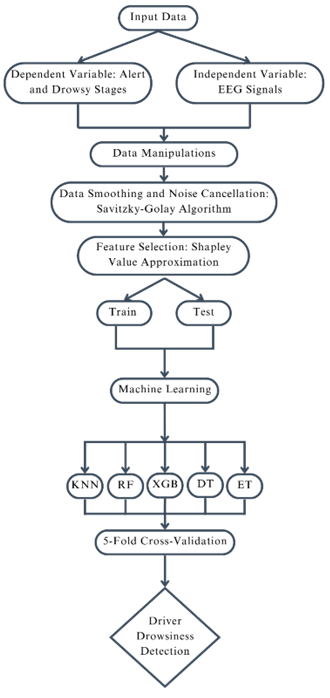
\includegraphics[width=7.2cm,keepaspectratio=true]{Fig_system_layout.png}
\vspace{-0.2cm}
\caption{\scriptsize Proposed System Layout.
\label{Fig_system_layout}}
\vspace{-0.3cm}
\end{figure}

The computed path loss is then used as the input features of the WCE localization system and the real mapped positions of the WCE are used as the output labels. The input and output datasets are then split into training and test datasets using the k-fold cross-validation and applied to the LSTM neural network for WCE localization.

\vspace{-0.2cm}
\section{Data Source}
\vspace{-0.1cm}
\subsection{Dataset Description}
An open EEG dataset released in 2019 by Cao et al. was used in our study. The study involved 27 voluntary participants aged 22–28 years, consisting of National Chiao Tung University students and staff. They participated in a 90-minute sustained-attention driving task multiple times on the same or different days, resulting in 62 EEG datasets. Participants were required to have normal or corrected-to-normal vision and no history of sleep deprivation, drug abuse, or irregular sleep patterns prior to the experiments. They avoided alcohol, caffeine, and strenuous exercise a day before the experiments. A VR driving environment was created using a dynamic driving simulator mounted on a six-degree-of-freedom Stewart motion platform. Six interactive highway driving scenes synchronized over local area networks were projected onto the screens at viewing angles of 0°, 42°, 84°, 180°, 276°, and 318° to provide a nearly complete 360° visual field.  An event-related lane-departure paradigm3 was implemented in the VR-based driving simulator using WorldToolKit (WTK) R9 Direct and Visual C++.  The driving task involved a visually monotonous night on a straight four-lane highway that mirrors real-life driving conditions. The lane-departure paradigm measured participants' reaction times to perturbations during a continuous driving task. Participants were instructed to keep the car in the center of the lane and respond to random lane-departure events by steering the car back to the original lane. The task lasted 90 minutes without breaks, and participants' activities were monitored via a surveillance video camera.

\begin{figure}[t!]
%\small 
\centering
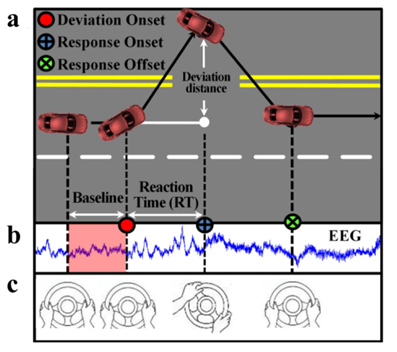
\includegraphics[width=7.2cm,keepaspectratio=true]{Fig_data_scenario.png}
\vspace{-0.2cm}
\caption{\scriptsize Experimental design,(a)	Event-related lane-deviation task. (b, c) Simultaneous EEG and behavioral recording.
\label{Fig_data_scenario}}
\vspace{-0.3cm}
\end{figure}
As shown in \ref{Fig_data_scenario}(a), lane-departure events were randomly induced to make the car drift from the original cruising lane towards the left or right sides (deviation onset). Each participant was instructed to quickly compensate for this perturbation by steering the wheel (response onset) to cause the car to move back to the original cruising lane (response offset). To avoid the impacts of other factors during the task, participants only reacted to the lane-perturbation event by turning the steering wheel. They did not have to control the accelerator or brake pedals in this experiment. Each lane-departure event was defined as a “trial,” including a baseline period, deviation onset, response onset, and response offset. EEG signals were recorded simultaneously \ref{Fig_data_scenario}(b).
The corresponding directions for turning the steering wheel are shown in \ref{Fig_data_scenario}(c) Of note, the next trial occurred within a 5–10 second interval after finishing the current trial, during which the subject had to maneuver the car back to the center line of the third car lane. If the participant fell asleep during the experiment, no feedback was provided to alert him/her.

\subsection{Electrode Layout in EEG Cap and Data Recording}
\begin{figure}[t!]
%\small 
\centering
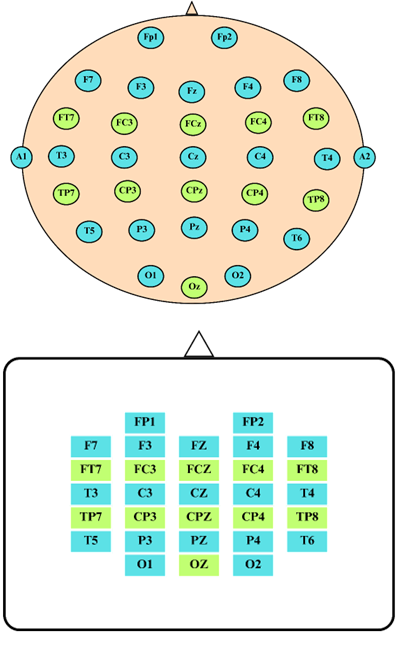
\includegraphics[width=7.2cm,keepaspectratio=true]{Fig_data_electrode.png}
\vspace{-0.2cm}
\caption{\scriptsize EEG Cap Electrode Layout where Blue electrodes represent the 10–20 system, and green indicates additional electrodes. Contact impedance was maintained below 5 $k\Omega$ for all electrodes. \label{Fig_data_electrode}}
\end{figure}

EEG data were recorded using a Scan SynAmps2 Express system with 32 Ag/AgCl electrodes as shown in Figure \ref{Fig_data_electrode} and were digitized at 500 Hz. The stimulus computer recorded Vehicle trajectories and events in a log file, which synchronized triggers with the EEG acquisition system. The data were integrated into a new file and imported into EEGLAB in MATLAB.
The EEG signals included 32 channels from electrodes placed according to a modified international 10–20 system. The recordings were analyzed using the EEGLAB toolbox in MATLAB, and events were classified as deviation onset, response onset, or response offset.
The first 32 signals were from the Fp1, Fp2, F7, F3, Fz, F4, F8, FT7, FC3, FCZ, FC4, FT8, T3, C3, Cz, C4, T4, TP7, CP3, CPz, CP4, TP8, A1, T5, P3, PZ, P4, T6, A2, O1, Oz and O2 electrodes. Two electrodes (A1 and A2) were references placed on the mastoid bones. The 33rd signal was used to describe the position of the simulated vehicle. A wired EEG cap with 30 EEG electrodes and two reference electrodes, placed according to a modified international 10–20 system, sampled the EEG signals at 500 Hz throughout the experiment.

\subsection{Data Extraction}
The dataset has already been preprocessed by its authors in the following steps:
\begin{enumerate}
\item The raw EEG signals were filtered by 1-Hz high-pass and 50-Hz low-pass finite impulse response (FIR) filters.
\item For artifact rejection, apparent eye blink contamination was manually removed. Ocular and muscular artifacts were removed using the Automatic Artifact Removal (AAR) plug-in provided in EEGLAB.
\item The original data was further down-sampled from 500 Hz to 128 Hz. 3s-long EEG samples were extracted prior to deviation onset for each trial. 
\end{enumerate}
\section{Methodologies}
\vspace{-0.1cm}
\subsection{Data manipulation and Results}
\vspace{-0.15cm}
\subsubsection{Segregation}
\begin{itemize}
    \item The EEG samples are segregated into alert and drowsy states for all the subjects based on the 'substate' variable.
    \item The segregated alert and drowsy data are saved into new '.mat' files.
    \end{itemize}
\subsubsection{Manipulating alert and drowsy state data}
\begin{itemize}
\item The alert data is loaded and transposed, concatenating all EEG samples into a new data frame.
\item Similar manipulation is performed on the drowsy state data.
\end{itemize}
\subsubsection{Creating Combined Dataset} The manipulated alert and drowsy datasets are concatenated row-wise into a new data frame.

Prior to manipulation, the initial EEG dataset contained 2022 samples, each with 30 channels and 384 data points, recorded over 3 seconds at a sampling rate of 128Hz from 11 subjects. The shape of each alert and drowsy states dataset was (1011, 384, 30) [1]. 

After manipulation, the dataset was transformed into a flat structure with 776448 rows and 31 columns where the additional column represented the 'substate' variable, which contains alert (0) and drowsy (1) states. This manipulation resulted in a new data frame for both alert and drowsy states, each with a shape of (388224, 31).
\begin{figure}[t!]
%\small 
\centering
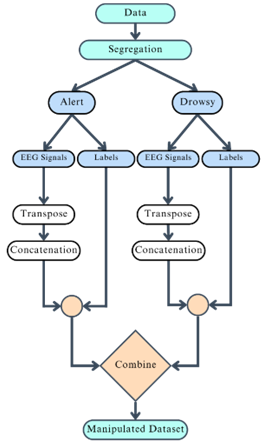
\includegraphics[width=7cm,keepaspectratio=true]{Fig_data_manipulation.png}
\vspace{-0.2cm}
\caption{\scriptsize Flowchart of the Data Manipulation Methodology.
\label{Fig_data_manipulation}}
\vspace{-0.3cm}
\end{figure}
%\begin{figure*}[t!]
%\small 
%\centering
%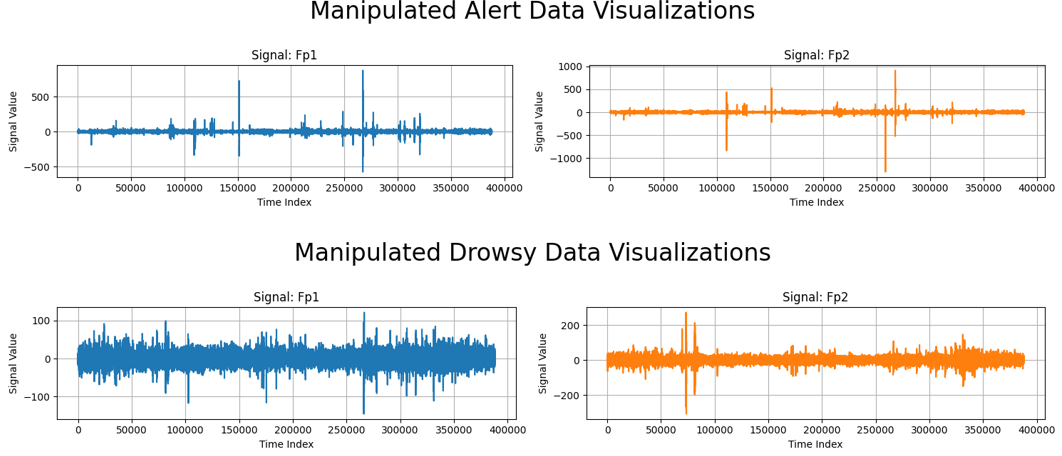
\includegraphics[width=17cm,keepaspectratio=true]{Fig_data_manip_results.PNG}
%\vspace{-0.2cm}
%\caption{\scriptsize Visualization of Manipulated Alert and Drowsy Data for Signal Fp1 and Fp2.
%\label{Fig_data_manip_results}}
%\vspace{-0.3cm}
%\end{figure*}
\begin{figure*}[t!]
%\small 
\centering
\lfbox[margin=0mm,border-style=none,padding=0mm,vertical-align=top]%{\includegraphics[width=6.5in,height=3.839in]
{\includegraphics[width=16cm,keepaspectratio=true]{Fig_data_smooth_alert.png}}
%\includegraphics[width=12cm,keepaspectratio=true]
\vspace{-0.2cm}
\caption{\scriptsize Alert data visualization for Manipulated unfiltered EEG signals vs. filtered EEG signals of Oz electrode.
\label{Fig_data_smooth_alert}}
\end{figure*}
\begin{figure*}[t!]
%\small 
\centering
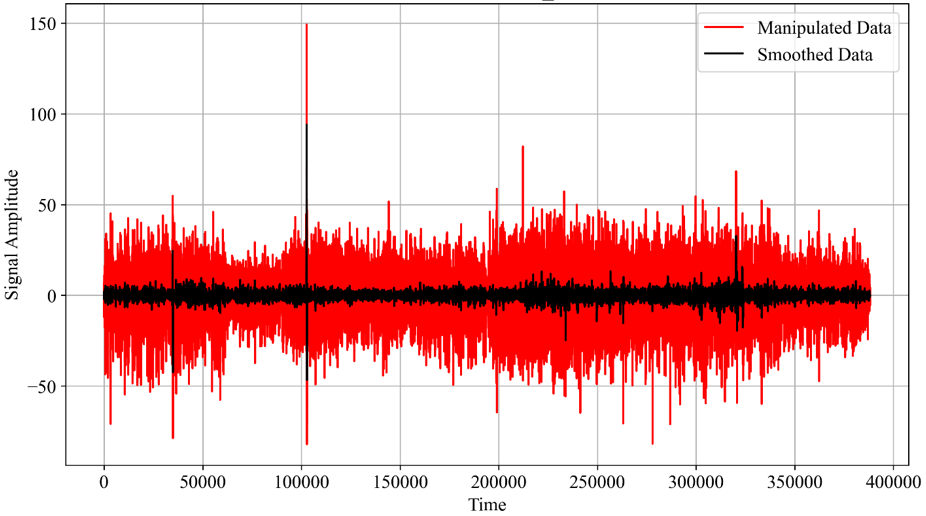
\includegraphics[width=16cm,keepaspectratio=true]{Fig_data_smooth_drowsy.png}
\vspace{-0.2cm}
\caption{\scriptsize Drowsy data visualization for Manipulated unfiltered EEG signals vs. filtered EEG signals of Oz electrode.
\label{Fig_data_smooth_drowsy}}
\end{figure*}
\subsection{Savitzky-Golay Data smoothing}
\vspace{-0.18cm}
To minimize the data deviations, we apply Savitzky–Golay (SG) filter to increase the precision of data without distorting the signal information. Savitzky–Golay filter is a digital filter that can be applied to a set of digital data points for the purpose of data smoothing. This is achieved using convolution process by fitting the successive sub-sets of adjacent data points with a low-degree polynomial by the method of linear least squares \cite{}. For smoothing by a m-point quadratic polynomial, the 
$j^{th}$ smoothed data point, $Y_j$ is given by
\vspace{-0.18cm}
\begin{eqnarray}
Y_{j}=&\sum^{\frac{m-1}{2}}_{i=-\frac{m-1}{2}} C_{i}y_{j+i} \label{eq_LOES}~,~~~~~~~~~\frac{m+1}{2}<= j<= \frac{m-1}{2}
\end{eqnarray}
where, $y_j$ are the original data values and $Y_j$ is the $j^{th}$ smoothed data point which is found using selected values of m convolution coefficients, 
$C_i$. 

\begin{table}[t!]
\centering
\caption{\scriptsize Performance using LSTM on the UWB path loss.}\label{tab:tab4}
\vspace{-0.2cm}
%\renewcommand{\arraystretch}{0.9}
\centering
\begin{tabular}
{|{c}|{c}|{c}|{c}|}
\hline
{\bfseries Window Size} &{\bfseries Polyorder = 1} &{\bfseries Polyorder = 3} &{\bfseries Polyorder = 5} \\\hline
 43 &
 0.9899 &
 0.9685 &
0.9398 \\\hline
 63 &
 0.9948 &
 0.9860 & 0.9687 \\\hline
 83 &
 0.9966 &
 0.9920 & 0.9824\\\hline
 93 &
 0.9974 &
 0.9936 &
 0.9860\\\hline
 103 &
 0.9978 &
 0.9948 &
 0.9884\\\hline
 123 &
 0.9977 &
 0.9964 &
 0.9927\\\hline
 143 &
 0.9980 &
 0.9977 &
 0.9945\\\hline
 163 &
 0.9981 &
 0.9982 &
 0.9959\\\hline
 203 &
 0.9985 &
 0.9987 &
 0.9975\\\hline
\end{tabular}
\end{table}
\subsubsection[Table: Altering window size and polynomial order with KNN accuracy to find the optimal
values.]{\textbf{Table: }Altering window size and polynomial order with KNN accuracy to find the optimal values.}
\begin{figure}
\centering
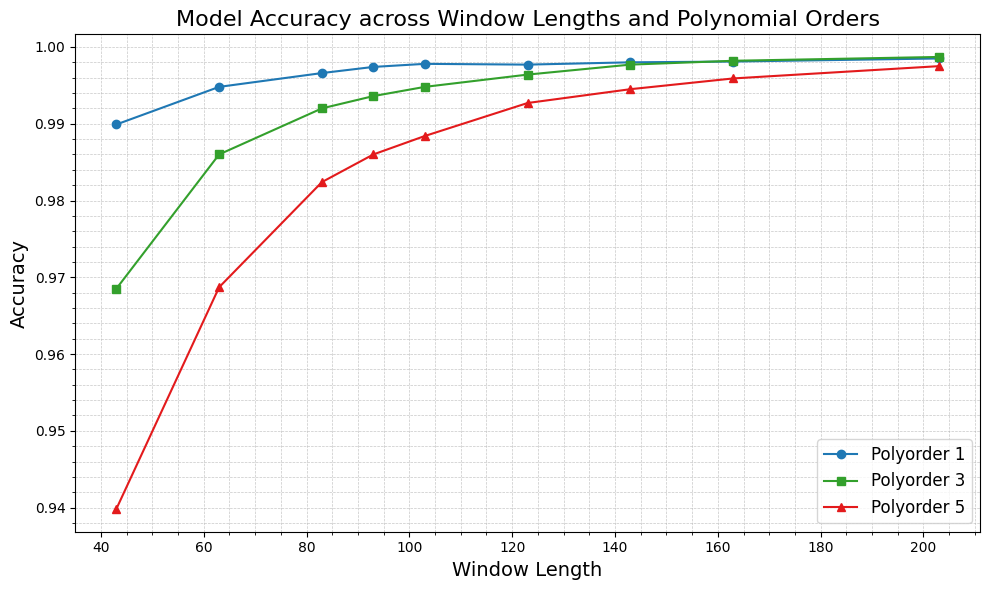
\includegraphics[width=8cm,keepaspectratio=true]{a0000-img008.png}
\vspace{-0.2cm}
\caption{\scriptsize KNN model accuracy across different window lengths and polynomial orders.
\label{a0000-img008}}
\end{figure}


\subsubsection[Figure: KNN model accuracy across different window lengths and polynomial
orders]{\textstyleInternetlink{\textbf{\textcolor[HTML]{1F3763}{Figure:}}\textcolor[HTML]{1F3763}{ KNN model accuracy
across different window lengths and polynomial orders}}}

\bigskip


\bigskip

\begin{figure*}[t!]
%\small 
\centering
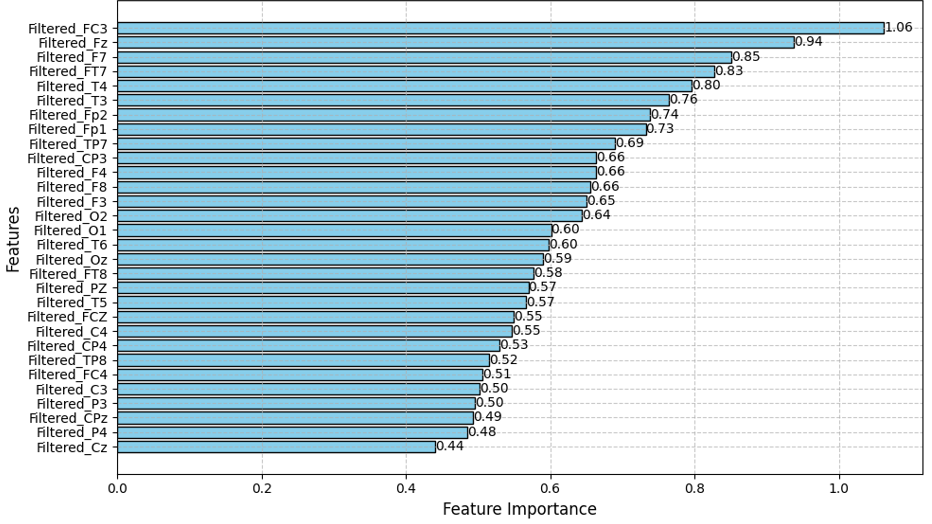
\includegraphics[width=16cm,keepaspectratio=true]{Fig_shapley.PNG}
\vspace{-0.2cm}
\caption{\scriptsize Feature Importance SHAP Values.}
\label{Fig_shapley}
\vspace{-0.2cm}
\end{figure*}
\begin{figure}[!t]
%\small 
\centering
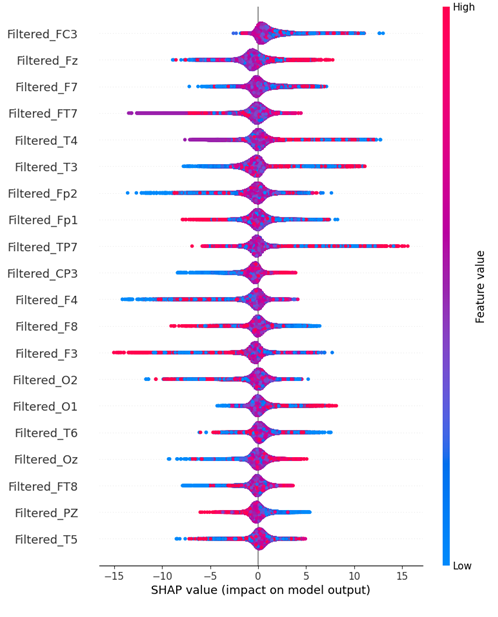
\includegraphics[width=8.6cm,keepaspectratio=true]{Fig_shapley_summart.png}
\vspace{-0.2cm}
\caption{\scriptsize SHAP summary Plot for Feature Impact Distribution using XGBoost model.}
\label{Fig_shapley_summart}
\vspace{-0.2cm}
\end{figure}
Figures \ref{Fig_data_smooth_alert} and \ref{Fig_data_smooth_drowsy} show the unfiltered and filtered original and smoothed EEG signals of Oz electrodes for the Alert and Drowsy case datasets. It is observed from the Figures \ref{Fig_data_smooth_alert} and \ref{Fig_data_smooth_drowsy} that the data deviations has been minimized significantly using the Savitzky–Golay data smoothing.
\subsection{Feature selection} 
The dataset is split into training and testing sets, with 80\% for training and 20\% for testing. XGBoost classifier is trained on the training data. GPU acceleration is utilized for faster computation, and the number of trees is set to 5000. SHAP is employed for interpreting the XGBoost model predictions. SHAP values are calculated for the test dataset to understand the contribution of each feature to the model's output. Feature importance is determined based on the absolute mean SHAP values across all instances in the test dataset.

A horizontal bar plot is created to illustrate the importance of each feature, with annotations showing the numerical values of importance.

A summary plot is generated to visualize the distribution of SHAP values for each feature.
\subsection{k-fold Cross validation}
\vspace{-0.15cm}
The k-fold cross-validation is applied to split the datasets and to validate the test accuracy of all the datasets \cite{175}. We apply 5-fold cross-validation where the datasets are shuffled to 42 random states and split into 5 groups each containing 20\% of the total datasets. Then one of the groups is taken as the test dataset and the remaining groups are taken as the training dataset. Then the proposed model is fitted on the training datasets and evaluated on the test datasets. Finally, the evaluation score is recorded for each test group and averaged to evaluate the performance of the model.
\vspace{-0.3cm}
\subsection{Machine Learning models}
\vspace{-0.15cm}
LSTM is a recurrent neural network (RNN), suitable to handle and train sequences of data as path loss using gradient-based optimization. The proposed LSTM architecture as shown in Figure \ref{Fig_LSTM_arch} consists of three LSTM layers followed by two fully connected dense layers. Batch normalization and ReLU activation are applied to enhance the model's training. The first LSTM layer with 512 units processes the input sequences, the second layer with 256 units returns sequences of hidden states for each time step and the third layer with 128 units does not return sequences and provides the final output for the last time step. The fully connected dense layers are added after the LSTM layers to further process the extracted features. The first dense layer has 64 units and the final dense layer is the output layer.
\vspace{-0.3cm}
\section{Simulation and Results}
\vspace{-0.1cm}
\subsection{Performance evaluation metric}
\vspace{-0.15cm}
The Root Mean Squared Error (RMSE) is calculated  by finding the square root of the average of the squared differences between the predicted and expected 3D locations of the target as follows
\vspace{-0.15cm}
\begin{eqnarray}
\textit{RMSE} &=&\sqrt{\frac{1}{M}\sum^{M}_{j}(P_j - \hat{P}_j)^2}
\vspace{-0.7cm}
\end{eqnarray}
where $P_j$ is the $j^$ expected real x-y-z {th}coordinate positions of the WCE in the dataset and $\hat{P}_{j}$ is the $j^{th}$ predicted positions.
\vspace{-0.3cm}
\subsection{Simulation results}
\vspace{-0.15cm}
The computational environment is based on a 64-bit Windows operating system with an x64-based Intel(R) Core(TM) i7-12700 CPU with 2.10 GHz processor, 32.00 GB RAM and NVIDIA GeForce RTX 3070 GPU. The RNN using LSTM is implemented using the TensorFlow and Keras libraries in Python. Adam optimizer with a learning rate of 0.0001 is used, and the mean squared error (MSE) loss function is selected. The model is trained using a 5-fold cross-validation approach with a batch size of 6. Early stopping with a patience of 30 is implemented to prevent overfitting and restore the best weights based on validation loss.


\subsection{Accuracy Metrics Table}
%\begin{flushleft}
\begin{table*}[t!]
\centering
\caption{\scriptsize Performance using LSTM on the UWB path loss.}\label{tab:tab4}
\vspace{-0.2cm}
%\renewcommand{\arraystretch}{0.9}
\begin{tabular}{|m{0.7677598in}|m{0.41085985in}|m{1.0830599in}|m{0.66565984in}|m{0.9497598in}|m{0.8309598in}|}
\hline
{\bfseries Feature} &
{\bfseries KNN} &
{\bfseries Random Forest} &
{\bfseries XGBoost} &
{\bfseries Decision Tree} &
{\bfseries Extra Trees}\\\hline
{\bfseries Feature 5} &
0.58 &
0.61 &
0.61 &
0.55 &
0.61\\\hline
{\bfseries Feature 8} &
0.61 &
0.65 &
0.65 &
0.57 &
0.64\\\hline
{\bfseries Feature 16} &
0.68 &
0.70 &
0.71 &
0.60 &
0.69\\\hline
{\bfseries Feature 22} &
0.69 &
0.71 &
0.72 &
0.60 &
0.69\\\hline
{\bfseries Feature 30} &
0.70 &
0.71 &
0.73 &
0.61 &
0.69\\\hline
\end{tabular}
\end{table*}
%\end{flushleft}

\begin{table*}[t!]
\centering
\caption{\scriptsize Performance using LSTM on the UWB path loss.}\label{tab:tab4}
\vspace{-0.2cm}
%\renewcommand{\arraystretch}{0.9}
\begin{tabular}{|m{0.7677598in}|m{0.49135986in}|m{1.0830599in}|m{0.66565984in}|m{0.9497598in}|m{0.8309598in}|}
\hline
{\bfseries Feature} &
{\bfseries KNN} &
{\bfseries Random Forest} &
{\bfseries XGBoost} &
{\bfseries Decision Tree} &
{\bfseries Extra Trees}\\\hline
{\bfseries Feature 5} &
0.9037 &
774.2472 &
3.7172 &
25.1586 &
130.6855\\\hline
{\bfseries Feature 8} &
1.2688 &
790.3788 &
4.2159 &
40.8654 &
143.5649\\\hline
{\bfseries Feature 16} &
0.0310 &
1593.1800 &
5.0250 &
90.0796 &
211.1900\\\hline
{\bfseries Feature 22} &
0.0518 &
1636.6767 &
5.5533 &
125.3308 &
219.2712\\\hline
{\bfseries Feature 30} &
0.0319 &
2069.2782 &
6.7332 &
168.4359 &
251.6688\\\hline
\end{tabular}
\end{table*}
%\end{flushleft}
We generate the path loss and position data in MATLAB. The generated path loss data are smoothed using LWLR and applied to the LSTM to predict the 3-dimensional x-y-z position of the WCE using the 5-fold cross-validation method. We consider the regular sensor topology as shown in Figure \ref{Fig2_sensor_topology}(a) considering the sensor receivers are placed on a wearable sensor array or jacket. We also consider that the sensor receivers are placed on the body surface using irregular sensor topology as shown in Figure \ref{Fig2_sensor_topology}(b). For regular and irregular topologies, three (03) different dimensions of the sensor array and small intestine are considered for normal, overweight, and obese human body as shown in Table \ref{tab:tab0}. The impact of the number of sensor receivers or the number of input features on the accuracy of localization and the computational time are analyzed and illustrated in Figures \ref{Fig_sen}(a) and 5(b). It is observed in Figure \ref{Fig_sen} that using the scattered path loss, the RMSE reduces while the time increases slightly by increasing the number of features. It is also observed that using only 16 sensor receivers, the highest accuracy with lower computational time is achieved. Table \ref{tab:tab4} and \ref{tab:tab5} summarize the evaluation scores using 16 sensor receivers with UWB and MICS path loss models, respectively. It is observed that for all scenarios, significantly high accuracy with low computational time is obtained using LSTM on the smoothed path loss for WCE localization.
\vspace{-0.4cm}
\begin{figure}[t!]
%\small 
\centering
\includegraphics[width=7.2cm,keepaspectratio=true]{Fig 5 impact of sensors.png}
\vspace{-0.2cm}
\caption{\scriptsize Impact of the number of features on the accuracy and time.}
\label{Fig_sen}
\vspace{-0.3cm}
\end{figure}
\begin{table}[t!]
\centering
\caption{\scriptsize Performance using LSTM on the UWB path loss.}\label{tab:tab4}
\vspace{-0.2cm}
%\renewcommand{\arraystretch}{0.9}
\begin{tabular}{|c|c|c|}
\hline
 \begin{tabular}{@{}c@{}}\end{tabular}&\begin{tabular}{@{}c@{}}UWB Scattered\end{tabular}&UWB LWLR\\ \hline
%&Scattered&LWLR&Scattered&LWLR
 \begin{tabular}{@{}c@{}}Sensor Topologies\end{tabular}&\begin{tabular}{c|c}RMSE&Time\\(mm)&(s)\end{tabular}&\begin{tabular}{c|c}RMSE&Time\\(mm)&(s)\end{tabular}\\\hline\hline
\begin{tabular}{@{}c@{}}Regular Normal\end{tabular}&\begin{tabular}{c|c}3.86&231.19\end{tabular}&\begin{tabular}{c|c}0.28&399.18\end{tabular}\\\hline
\begin{tabular}{@{}c@{}}Regular Overweight\end{tabular}&\begin{tabular}{c|c}4.55&265.88\end{tabular}&\begin{tabular}{c|c}0.48&342.90\end{tabular}\\\hline
\begin{tabular}{@{}c@{}}Regular Obese\end{tabular}&\begin{tabular}{c|c}7.55&286.23\end{tabular}&\begin{tabular}{c|c}0.36&453.03\end{tabular}\\\hline
\begin{tabular}{@{}c@{}}Irregular Normal\end{tabular}&\begin{tabular}{c|c}3.74&347.55
%3.79&265.89
\end{tabular}&\begin{tabular}{c|c}0.24&467.77
%0.28&1093.25
\end{tabular}\\\hline
\begin{tabular}{@{}c@{}}Irregular Overweight\end{tabular}&\begin{tabular}{c|c}2.71&290.11\end{tabular}&\begin{tabular}{c|c}0.26&439.32\end{tabular}\\\hline
\begin{tabular}{@{}c@{}}Irregular Obese\end{tabular}&\begin{tabular}{c|c}3.98&303.75\end{tabular}&\begin{tabular}{c|c}0.29&413.96\end{tabular}\\\hline
  \end{tabular}
\vspace{-0.4cm}
\end{table}
\begin{table}[t!]
\centering
\caption{\scriptsize Performance using LSTM on the MICS path loss.}\label{tab:tab5}
\vspace{-0.2cm}
\begin{tabular}{|c|c|c|c|c|}
\hline
 \begin{tabular}{@{}c@{}}\end{tabular}&\begin{tabular}{@{}c@{}}MICS Scattered\end{tabular}&MICS LWLR\\\hline
%&Scattered&LWLR&Scattered&LWLR
 \begin{tabular}{@{}c@{}}Sensor Topologies\end{tabular}&\begin{tabular}{c|c}RMSE&Time\\(mm)&(s)\end{tabular}&\begin{tabular}{c|c}RMSE&Time\\(mm)&(s)\end{tabular}\\\hline\hline
\begin{tabular}{@{}c@{}}Regular Normal\end{tabular}&\begin{tabular}{c|c}19.09&211.5\end{tabular}&\begin{tabular}{c|c}0.38&409.59\end{tabular}\\\hline
\begin{tabular}{@{}c@{}}Regular Overweight\end{tabular}&\begin{tabular}{c|c}35.93&267.2\end{tabular}&\begin{tabular}{c|c}0.505&435.84\end{tabular}\\\hline
\begin{tabular}{@{}c@{}}Regular Obese\end{tabular}&\begin{tabular}{c|c}40.14&204.0\end{tabular}&\begin{tabular}{c|c}0.73&587.13\end{tabular}\\\hline
\begin{tabular}{@{}c@{}}Irregular Normal\end{tabular}&\begin{tabular}{c|c}18.02&220.9
%17.96&197.15
\end{tabular}&\begin{tabular}{c|c}0.27&532.23
%0.30&488.25
\end{tabular}\\\hline
\begin{tabular}{@{}c@{}}Irregular Overweight\end{tabular}&\begin{tabular}{c|c}19.29&220.1\end{tabular}&\begin{tabular}{c|c}0.35&422.69\end{tabular}\\\hline
\begin{tabular}{@{}c@{}}Irregular Obese\end{tabular}&\begin{tabular}{c|c}23.0&217.52\end{tabular}&\begin{tabular}{c|c}0.37&507.54\end{tabular}\\\hline 
  \end{tabular}
\vspace{-0.3cm}
\end{table}
\section{Conclusion}
\vspace{-0.13cm}
In this paper, we have proposed WCE localization using LSTM regression. We have generated the UWB and MICS path loss data for 2443 mapped positions in the small intestine for 6 sensor topologies and applied LSTM with 5-fold cross-validation for WCE localization. We have obtained RMSE of 0.24 $mm$ and 0.27 $mm$ in 467.77 sec and 532.23 sec time using only 16 sensor receivers with UWB and MICS channel models, respectively without any prior knowledge of the channel parameters, distance, reference positions, and bounds. 
\vspace{-0.2cm}
%\section*{Acknowledgment}
% addcontentsline needed when using bookmark hyperlinking, etc.
%\addcontentsline{toc}%{section}{Acknowledgment}
% enable scriptsize
%\scriptsize
%This work was supported by the resources provided by the Department of EEE, AUST.
%\normalsize
\bibliographystyle{IEEEtran}
%\vspace{-0.7cm}
\bibdata{IEEEabrv,sn-bibliography}
\bibliography{sn-bibliography}
%\bibitem{IEEEhowto:kopka}
%H.~Kopka and P.~W. Daly, \emph{Guide to \LaTeX}, 4th~ed.\hskip 1em plus
 % 0.5em minus 0.4em\relax Boston, MA: Addison-Wesley, 2004.
% that's all folks
\end{document}


